\chapter{}{{Experimental Results and Discussion}}{Experimental Results and Discussion}

As stated in Chapters 1 and 2, the experimental setup in the proposed approach differs from the standard ZSL setup. The proposed approach aims to minimize the number of seen classes within a data set while delivering reasonable performance on the unseen classes. This makes it hard to compare our results with those of other ZSL frameworks mentioned in the research literature. In order to achieve a fair comparison of the proposed framework with other ZSL approaches, we modify a well known ZSL framework to work with our experiment setup. 

\par
\medskip
 
\textbf{Attribute Label Embedding (ALE)} \cite{ale} uses a bi-linear compatibility function to associate visual and auxiliary information. It embeds each class in the space of attribute vectors. The approach also generalizes to any type of auxiliary information that can be encoded in matrix form such as word embeddings. A comparison study performed in \cite{gbu} shows that ALE outperforms other ZSL frameworks in the generalized ZSL setting. Recent generative methods described in the literature could potentially perform better than ALE but such a comparison study using same data sets, experimental conditions, and evaluation metrics has not been performed yet. Hence, we chose to compare the proposed approach with the ALE framework. A working implementation of the ALE framework was obtained from a recent GitHub repository \footnote{https://github.com/cetinsamet/attribute-label-embedding}
and modified to work within our experimental setting. Once the clusters centers are determined for each value of $k$, the ALE procedure is performed on the appropriate training and testing sets. Table~\ref{table:gmm_com} and Table~\ref{table:af_com} show a summary of the comparison between the proposed approach and ALE using both clustering techniques, i.e., GMM-based clustering and AP-based clustering. Table~\ref{table:full_results} in Appendix B provides comprehensive results on all three data sets when using GMM-based clustering.

\par
\medskip
\noindent 
\textbf{Results on the AWA2 data set.} The AWA2 data set has 50 classes and the training set consists of 560 images per class on average with the category \textit{horse} having the highest number of images (1316), and  the category \textit{mole} having the least number of images (80). 

We study performance of the proposed approach for $k = 25$ which renders half the classes as seen and half the classes as unseen for the model. The seen classes exhibit an average classification accuracy of 85\% whereas the unseen classes exhibit an average classification accuracy of 27\% on the test set. 

Among the seen classes, we find there are three cases:

\begin{enumerate}[label=Seen Case: \arabic*]
    \item Seen classes exhibiting $\geq 90\%$ classification accuracy on the test set. In the AWA2 data set, 16 of 25 seen classes fall in this category and are expected to aid very well in the inference of unseen classes related to these seen classes. These seen classes have a good number of images to train on and the classifier is able to clearly identify distinguishing features for each class. For example, \textit{humpback whale} is a seen class that exhibits 100\% classification accuracy on the test set. Ideally, we would want all seen classes to fall into this category.
    
    \item Seen classes exhibiting classification accuracy $\geq 60\%$ but $< 90\%$ on the test set. In the AWA2 data set, 7 of 25 seen classes fall in this category and are expected to aid reasonably in the inference of unseen classes. Although these classes have a reasonable number of images to train on, these classes fall into a case where the classes are very close to each other but are still seen classes. For example, \textit{ox}, \textit{moose}, and \textit{cow} fall in this category. It is understandable why the visual classifier would not be able to clearly distinguish between these categories, they are quite similar compared to other categories in this data set.  
    
    \item Seen classes exhibiting classification accuracy $ < 60\%$ on the test set. In the AWA2 data set, 2 of 25 seen classes fall in this category and are expected to negatively impact the unseen class inference process. These 2 classes have only an average of 160 images in the training set, hence the visual classifiers were not be trained enough on these classes to learn the discriminating features.
\end{enumerate}

\par
\medskip

Among the unseen classes also we find three cases:

\begin{enumerate}[label=Unseen Case: \arabic*]
    \item Unseen classes exhibiting $>60\%$  classification accuracy on the test set. In the AWA2 data set, 6 of 25 unseen classes fall in this category. These are cases when a particular unseen class is inferred from a seen class falling in Case 1 of seen classes. For example, \textit{blue whale} is an unseen class that exhibits 100\% accuracy on the test set, and it is inferred from \textit{humpback whale} which falls under Case 1 of the seen classes.
    
    \item Unseen classes exhibiting classification accuracy $\geq  1\%$  but $\leq 60\%$ on the test set. In the AWA2 data set, 6 of 25 unseen classes fall in this category. These are cases where the unseen classes are inferred from the seen classes falling in Case 2 and Case 3 of seen classes. These unseen classes exhibit poor performance since the seen classes they are inferred from are not clearly distinguishable by the visual classifier. For example, \textit{deer} is an unseen class that is inferred from the seen class \textit{moose} which falls in Case 2 of the seen classes.
    
    \item Unseen classes that exhibit $0\%$ accuracy on the test set. In the AWA2 data set, 12 of 25 unseen classes fall in this category. Since our inference process only allows for guessing 1 unseen class per seen class, unseen classes that are farther away from seen classes cannot be inferred and fall in this category. For example, \textit{antelope} is an unseen class that falls in the cluster of \textit{moose}, but only \textit{deer} can be inferred from \textit{moose} since it is the closest neighbor to \textit{moose} based on the cosine similarity measure.
\end{enumerate}

\par
\medskip

The proposed model performs well when a seen class has a sufficient number of images to train on and the unseen class being inferred from it is proximal to the seen class and it performs poorly when the unseen class being inferred is distant from any of the representative classes. Ideally, the proposed model would perform best when there are clusters of size 2 and the representative object for the cluster has clear discriminating features, while the unseen class in the cluster is also closer to the representative class than any other class. Figure~\ref{image:awa2_comparison} shows a comparison of the H-scores obtained on the AWA2 data set by the proposed model and ALE for all values of $k$. As seen from the graph, our model performs significantly better than ALE for all values of $k$ on this data set. The H-score keeps increasing as the value of $k$ increases which is expected since the number of seen classes increase which enables more unseen classes to be inferred more accurately. 

\par
\medskip

In order to determine the optimal numbers of classes required to achieve reasonable performance, we choose a $k$ value for which we achieve a greater than average H-score performance with the proposed model. For $k = 20$, we achieve a H-score of 46\% with the proposed model whereas the average H-score on the AWA2 data set is 45\% across all categories. Thus, on the AWA2 data set, we need to have at least 20 categories as seen classes to reasonably infer the unseen classes with greater than average accuracy with the proposed model.

\par
\medskip

\begin{figure}[h]
\centering
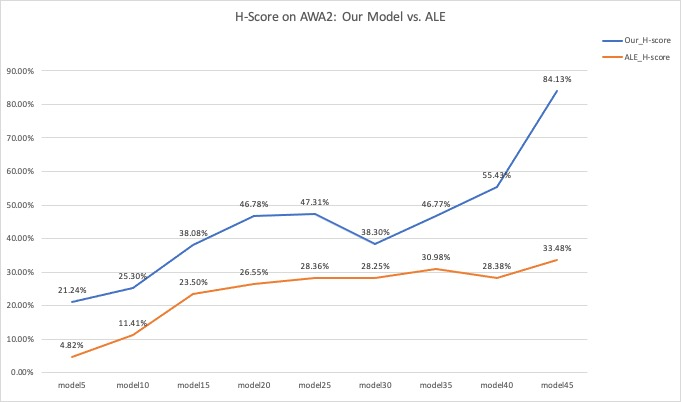
\includegraphics[width=\textwidth]{MS-Thesis-master/figures/awa2_comparison.jpg}
\caption{H-score comparison between the proposed model and ALE on AWA2 data set when using GMM-based clustering.}
\label{image:awa2_comparison}
\end{figure}

\par
\medskip
\noindent
\textbf{Results on the CUB data set.} The CUB data set has 200 classes with 47 images per class on average in the training set. This is a small number of images to train on for each seen class. However, the proposed model still performs well on this data set. 

\par
\medskip

Figure~\ref{image:cub_comparison} shows a comparison of H-scores obtained on the CUB data set using the proposed model and ALE for all values of $k$. As seen from the graph, the proposed model performs better than ALE for values of $k \leq 65$. For $65 < k \leq 115$, the proposed model and ALE exhibit comparable performance and for $k > 115$, the proposed model significantly outperforms ALE on the CUB data set. Thus, across a large range of $k$ values, the proposed model performs better than ALE on the CUB data set. 

\par
\medskip

For $k = 80$, we achieve a H-score of 33.5\% with the proposed model whereas the average H-score on the CUB data set is 33\% across all categories. Thus, on the CUB data set, we need to use at least 80 categories as seen classes to reasonably infer the unseen classes with higher than average accuracy with the proposed model.

\par
\medskip

\begin{figure}[h]
\centering
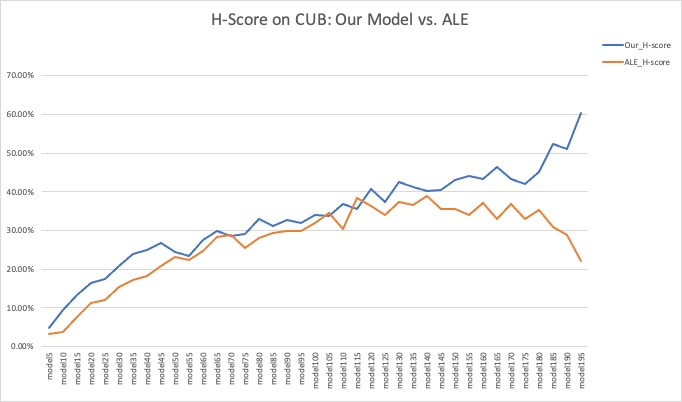
\includegraphics[width=\textwidth]{MS-Thesis-master/figures/cub_comparison.jpg}
\caption{H-score comparison between the proposed model and ALE on CUB data set when using GMM-based clustering.}
\label{image:cub_comparison}
\end{figure}

\par
\medskip
\noindent
\textbf{Results on the SUN data set.} The SUN data set has 717 classes with 16 images per class on average in the training set. This makes it hard for the visual classifier to learn distinguishing features for each class because of the large number of classes and small number of images for each class. Nevertheless, the proposed model exhibits performance that is comparable to ALE on this data set. Figure~\ref{image:sun_comparison} shows a comparison of H-scores obtained on the SUN data set using the proposed model and ALE for all values of $k$. As seen from the graph, ALE performs better than the proposed model for values of $k \leq 560$ and the proposed model performs better than ALE for values of $k$ beyond 560.

\par
\medskip

For $k = 360$, we achieve a H-score of 22\% with the proposed model and the average H-score on the CUB data set is 21.6\% across all categories. Thus, on the SUN data set, we need to use at least 360 categories as seen classes to reasonably infer the unseen classes with greater than average accuracy with the proposed model.

\par
\medskip

\begin{figure}[h]
\centering
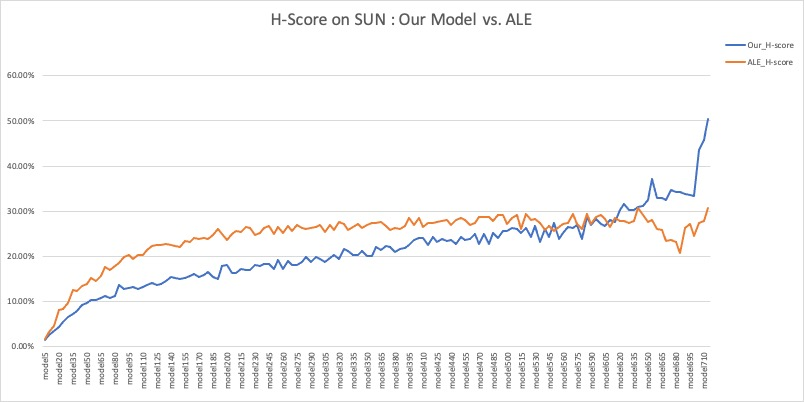
\includegraphics[width=\textwidth]{MS-Thesis-master/figures/sun_comparison.jpg}
\caption{H-score comparison between the proposed model and ALE on SUN data set when using GMM-based clustering.}
\label{image:sun_comparison}
\end{figure}

\par
\medskip

\begin{table}[h]
\caption{Comparison of average classification accuracy across $k$ values between the proposed model and ALE when using GMM-based clustering.}
\centering
\begin{tabular}{@{}lllllll@{}}
\toprule
\textbf{}        & \multicolumn{3}{c}{\textbf{Proposed Model}}                            & \multicolumn{3}{c}{\textbf{ALE}}                                  \\ \midrule
\textbf{Data Set} & \textbf{Avg. Seen} & \textbf{Avg. Unseen} & \textbf{Avg. H-Score} & \textbf{Avg. Seen} & \textbf{Avg. Unseen} & \textbf{Avg. H-Score} \\
AWA2             & 94\%               & 32\%                 & \textbf{45\%}         & 90\%               & 14\%                 & 24\%                  \\
CUB              & 78\%               & 22.86\%              & \textbf{33\%}         & 70\%               & 17.50\%              & 27.19\%               \\
SUN              & 58.20\%            & 15\%                 & 21.60\%               & 41.50\%            & 17.80\%              & \textbf{25\%}         \\ \bottomrule
\end{tabular}
\label{table:gmm_com}
\end{table}

\par
\medskip

\begin{table}[ht]
\caption{Comparison of average classification accuracy between the proposed model and ALE when using AP-based clustering.}
\centering
\begin{tabular}{@{}lllllll@{}}
\toprule
                 & \multicolumn{3}{c}{\textbf{Proposed Model}}             & \multicolumn{3}{c}{\textbf{ALE}}                   \\ \midrule
\textbf{Data Set} & \textbf{Seen} & \textbf{Unseen} & \textbf{H-Score} & \textbf{Seen} & \textbf{Unseen} & \textbf{H-Score} \\
AWA2             & 96.44\%          & 23.43\%         & \textbf{37.7\%}    & 83.40\%       & 10\%            & 17.50\%          \\
CUB              & 91\%          & 9.70\%          & \textbf{17.50\%} & 55\%          & 8.33\%          & 14.40\%          \\
SUN              & 83.10\%       & 4.30\%          & 8.20\%           & 24.40\%       & 8.20\%          & \textbf{12.30\%} \\ \bottomrule
\end{tabular}
\label{table:af_com}
\end{table}

\par
\bigskip
\bigskip
\noindent
\textbf{Hardware Specifications.} All the experiments were performed on an Intel I7 6850K CPU with 128GB RAM. For the AWA2 data set, it takes $\approx$ 20 minutes to train visual classifiers for all values of $k$.  Likewise, for the CUB and SUN data sets, it takes $\approx$ 2.5 hours and $\approx$ 40 hours, respectively, to train visual classifiers for all values of $k$.





\newpage